%%%%%%%%%%%%%%%%%%%%%%%%%%%%%%%%%%%%%%%%%
% Lachaise Assignment
% LaTeX Template
% Version 1.0 (26/6/2018)
%
% This template originates from:
% http://www.LaTeXTemplates.com
%
% Authors:
% Marion Lachaise & François Févotte
% Vel (vel@LaTeXTemplates.com)
%
% License:
% CC BY-NC-SA 3.0 (http://creativecommons.org/licenses/by-nc-sa/3.0/)
% 
%%%%%%%%%%%%%%%%%%%%%%%%%%%%%%%%%%%%%%%%%

%----------------------------------------------------------------------------------------
%	PACKAGES AND OTHER DOCUMENT CONFIGURATIONS
%----------------------------------------------------------------------------------------

\documentclass{article}

%%%%%%%%%%%%%%%%%%%%%%%%%%%%%%%%%%%%%%%%%
% Lachaise Assignment
% Structure Specification File
% Version 1.0 (26/6/2018)
%
% This template originates from:
% http://www.LaTeXTemplates.com
%
% Authors:
% Marion Lachaise & François Févotte
% Vel (vel@LaTeXTemplates.com)
%
% License:
% CC BY-NC-SA 3.0 (http://creativecommons.org/licenses/by-nc-sa/3.0/)
% 
%%%%%%%%%%%%%%%%%%%%%%%%%%%%%%%%%%%%%%%%%

%----------------------------------------------------------------------------------------
%	PACKAGES AND OTHER DOCUMENT CONFIGURATIONS
%----------------------------------------------------------------------------------------

\usepackage{amsmath,amsfonts,stmaryrd,amssymb} % Math packages

\usepackage{enumerate} % Custom item numbers for enumerations

\usepackage{subcaption}
\usepackage{cleveref}
\usepackage[ruled]{algorithm2e} % Algorithms

\usepackage[framemethod=tikz]{mdframed} % Allows defining custom boxed/framed environments

\usepackage{listings} % File listings, with syntax highlighting
\lstset{
	basicstyle=\ttfamily, % Typeset listings in monospace font
}

%----------------------------------------------------------------------------------------
%	DOCUMENT MARGINS
%----------------------------------------------------------------------------------------

\usepackage{geometry} % Required for adjusting page dimensions and margins

\geometry{
	paper=a4paper, % Paper size, change to letterpaper for US letter size
	top=2.5cm, % Top margin
	bottom=3cm, % Bottom margin
	left=2.5cm, % Left margin
	right=2.5cm, % Right margin
	headheight=14pt, % Header height
	footskip=1.5cm, % Space from the bottom margin to the baseline of the footer
	headsep=1.2cm, % Space from the top margin to the baseline of the header
	%showframe, % Uncomment to show how the type block is set on the page
}

%----------------------------------------------------------------------------------------
%	FONTS
%----------------------------------------------------------------------------------------

\usepackage[utf8]{inputenc} % Required for inputting international characters
\usepackage[T1]{fontenc} % Output font encoding for international characters

%\usepackage{XCharter} % Use the XCharter fonts

%----------------------------------------------------------------------------------------
%	COMMAND LINE ENVIRONMENT
%----------------------------------------------------------------------------------------

% Usage:
% \begin{commandline}
%	\begin{verbatim}
%		$ ls
%		
%		Applications	Desktop	...
%	\end{verbatim}
% \end{commandline}

\mdfdefinestyle{commandline}{
	leftmargin=10pt,
	rightmargin=10pt,
	innerleftmargin=15pt,
	middlelinecolor=black!50!white,
	middlelinewidth=2pt,
	frametitlerule=false,
	backgroundcolor=black!5!white,
	frametitle={Command Line},
	frametitlefont={\normalfont\sffamily\color{white}\hspace{-1em}},
	frametitlebackgroundcolor=black!50!white,
	nobreak,
}

% Define a custom environment for command-line snapshots
\newenvironment{commandline}{
	\medskip
	\begin{mdframed}[style=commandline]
}{
	\end{mdframed}
	\medskip
}

%----------------------------------------------------------------------------------------
%	FILE CONTENTS ENVIRONMENT
%----------------------------------------------------------------------------------------

% Usage:
% \begin{file}[optional filename, defaults to "File"]
%	File contents, for example, with a listings environment
% \end{file}

\mdfdefinestyle{file}{
	innertopmargin=1.6\baselineskip,
	innerbottommargin=0.8\baselineskip,
	topline=false, bottomline=false,
	leftline=false, rightline=false,
	leftmargin=2cm,
	rightmargin=2cm,
	singleextra={%
		\draw[fill=black!10!white](P)++(0,-1.2em)rectangle(P-|O);
		\node[anchor=north west]
		at(P-|O){\ttfamily\mdfilename};
		%
		\def\l{3em}
		\draw(O-|P)++(-\l,0)--++(\l,\l)--(P)--(P-|O)--(O)--cycle;
		\draw(O-|P)++(-\l,0)--++(0,\l)--++(\l,0);
	},
	nobreak,
}

% Define a custom environment for file contents
\newenvironment{file}[1][File]{ % Set the default filename to "File"
	\medskip
	\newcommand{\mdfilename}{#1}
	\begin{mdframed}[style=file]
}{
	\end{mdframed}
	\medskip
}

%----------------------------------------------------------------------------------------
%	NUMBERED QUESTIONS ENVIRONMENT
%----------------------------------------------------------------------------------------

% Usage:
% \begin{question}[optional title]
%	Question contents
% \end{question}

\mdfdefinestyle{question}{
	innertopmargin=1.2\baselineskip,
	innerbottommargin=0.8\baselineskip,
	roundcorner=5pt,
	nobreak,
	singleextra={%
		\draw(P-|O)node[xshift=1em,anchor=west,fill=white,draw,rounded corners=5pt]{%
		Question \theQuestion\questionTitle};
	},
}

\newcounter{Question} % Stores the current question number that gets iterated with each new question

% Define a custom environment for numbered questions
\newenvironment{question}[1][\unskip]{
	\bigskip
	\stepcounter{Question}
	\newcommand{\questionTitle}{~#1}
	\begin{mdframed}[style=question]
}{
	\end{mdframed}
	\medskip
}

%----------------------------------------------------------------------------------------
%	WARNING TEXT ENVIRONMENT
%----------------------------------------------------------------------------------------

% Usage:
% \begin{warn}[optional title, defaults to "Warning:"]
%	Contents
% \end{warn}

\mdfdefinestyle{warning}{
	topline=false, bottomline=false,
	leftline=false, rightline=false,
	nobreak,
	singleextra={%
		\draw(P-|O)++(-0.5em,0)node(tmp1){};
		\draw(P-|O)++(0.5em,0)node(tmp2){};
		\fill[black,rotate around={45:(P-|O)}](tmp1)rectangle(tmp2);
		\node at(P-|O){\color{white}\scriptsize\bf !};
		\draw[very thick](P-|O)++(0,-1em)--(O);%--(O-|P);
	}
}

% Define a custom environment for warning text
\newenvironment{warn}[1][Warning:]{ % Set the default warning to "Warning:"
	\medskip
	\begin{mdframed}[style=warning]
		\noindent{\textbf{#1}}
}{
	\end{mdframed}
}

%----------------------------------------------------------------------------------------
%	INFORMATION ENVIRONMENT
%----------------------------------------------------------------------------------------

% Usage:
% \begin{info}[optional title, defaults to "Info:"]
% 	contents
% 	\end{info}

\mdfdefinestyle{info}{%
	topline=false, bottomline=false,
	leftline=false, rightline=false,
	nobreak,
	singleextra={%
		\fill[black](P-|O)circle[radius=0.4em];
		\node at(P-|O){\color{white}\scriptsize\bf i};
		\draw[very thick](P-|O)++(0,-0.8em)--(O);%--(O-|P);
	}
}

% Define a custom environment for information
\newenvironment{info}[1][Info:]{ % Set the default title to "Info:"
	\medskip
	\begin{mdframed}[style=info]
		\noindent{\textbf{#1}}
}{
	\end{mdframed}
}
 % Include the file specifying the document structure and custom commands

%----------------------------------------------------------------------------------------
%	ASSIGNMENT INFORMATION
%----------------------------------------------------------------------------------------

\title{CS6910: Programming Assignment 1} % Title of the assignment

\author{Vimarsh Sathia\\ \texttt{CS17B046}} % Author name and email address

\date{Indian Institute of Technology Madras --- \today} % University, school and/or department name(s) and a date

%----------------------------------------------------------------------------------------

\begin{document}

\maketitle % Print the title

%----------------------------------------------------------------------------------------
%	INTRODUCTION
%----------------------------------------------------------------------------------------
\section*{General Information}
All image classification experiments were carried out on the subset of the CIFAR-10 dataset provided in split $2$. Each input is a $3 \times 64 \times 64$ RGB image.\\
During the training phase in Part-A, batch size was taken to be $32$ for all $4$ models.

\section{Part-A}
For this part, $4$ different models(Net1, Net2, Net3 and Net4) with different network parameters were trained. The code defining the 4 neural network modules can be found in \lstinline!classifiers.py!. A brief summary of the network layers is shown in \cref{fig:models}.

\begin{figure}[h!]
	\begin{subfigure}[t]{.23\textwidth}
	  \centering
	  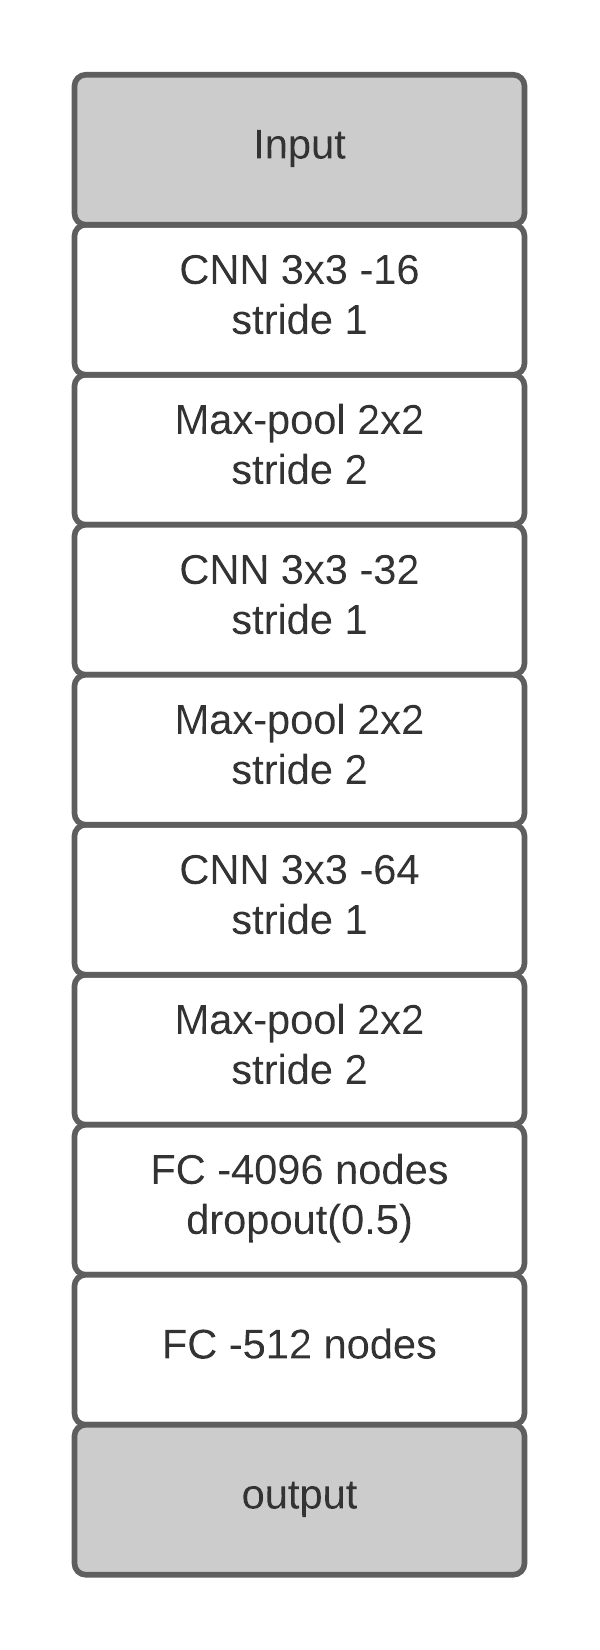
\includegraphics[scale=0.66]{../code/images/Net1_layers.png}  
	  \caption{Net1}
	\end{subfigure}
	\begin{subfigure}[t]{.23\textwidth}
	  \centering
	  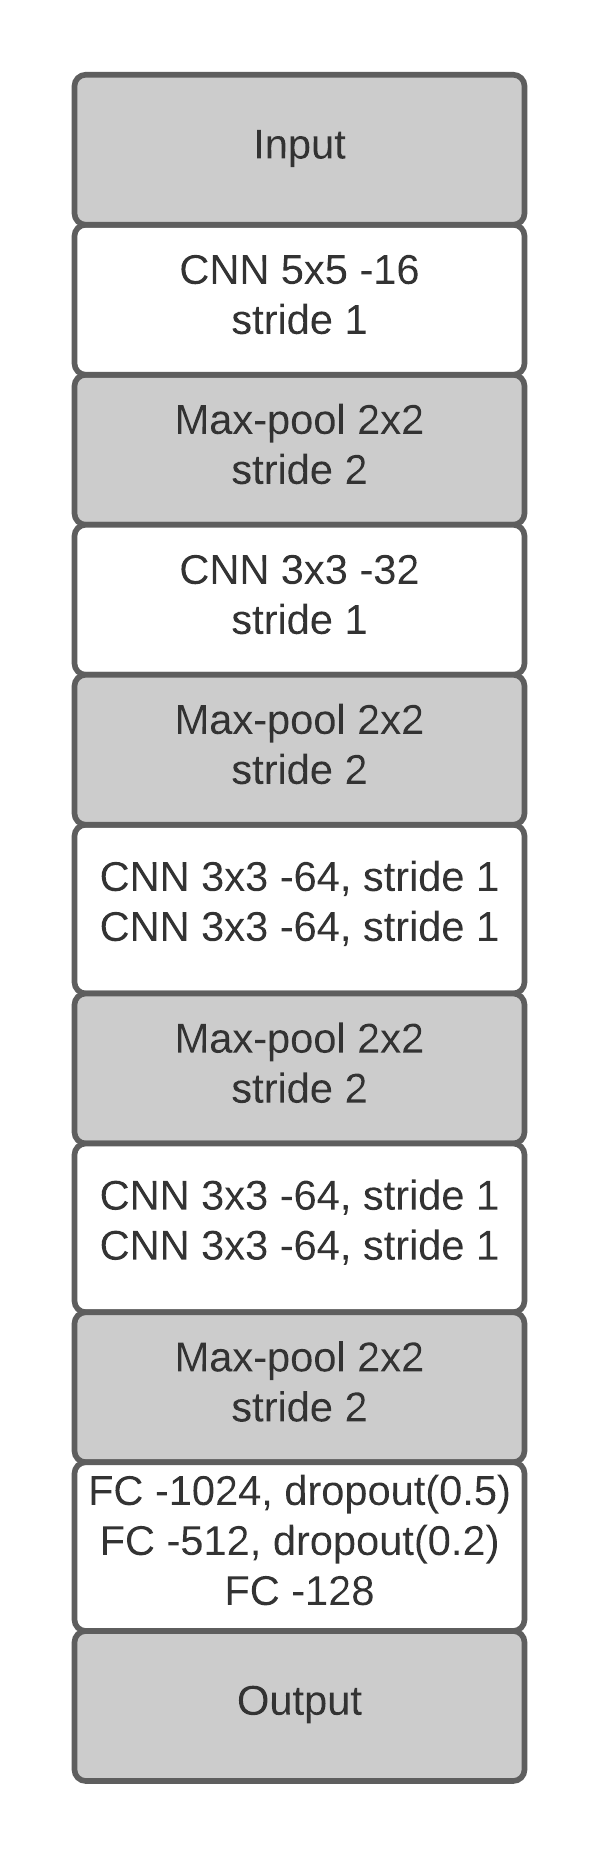
\includegraphics[scale=0.66]{../code/images/Net2_layers.png}  
	  \caption{Net2}
	\end{subfigure}
	\begin{subfigure}[t]{.23\textwidth}
	\centering
	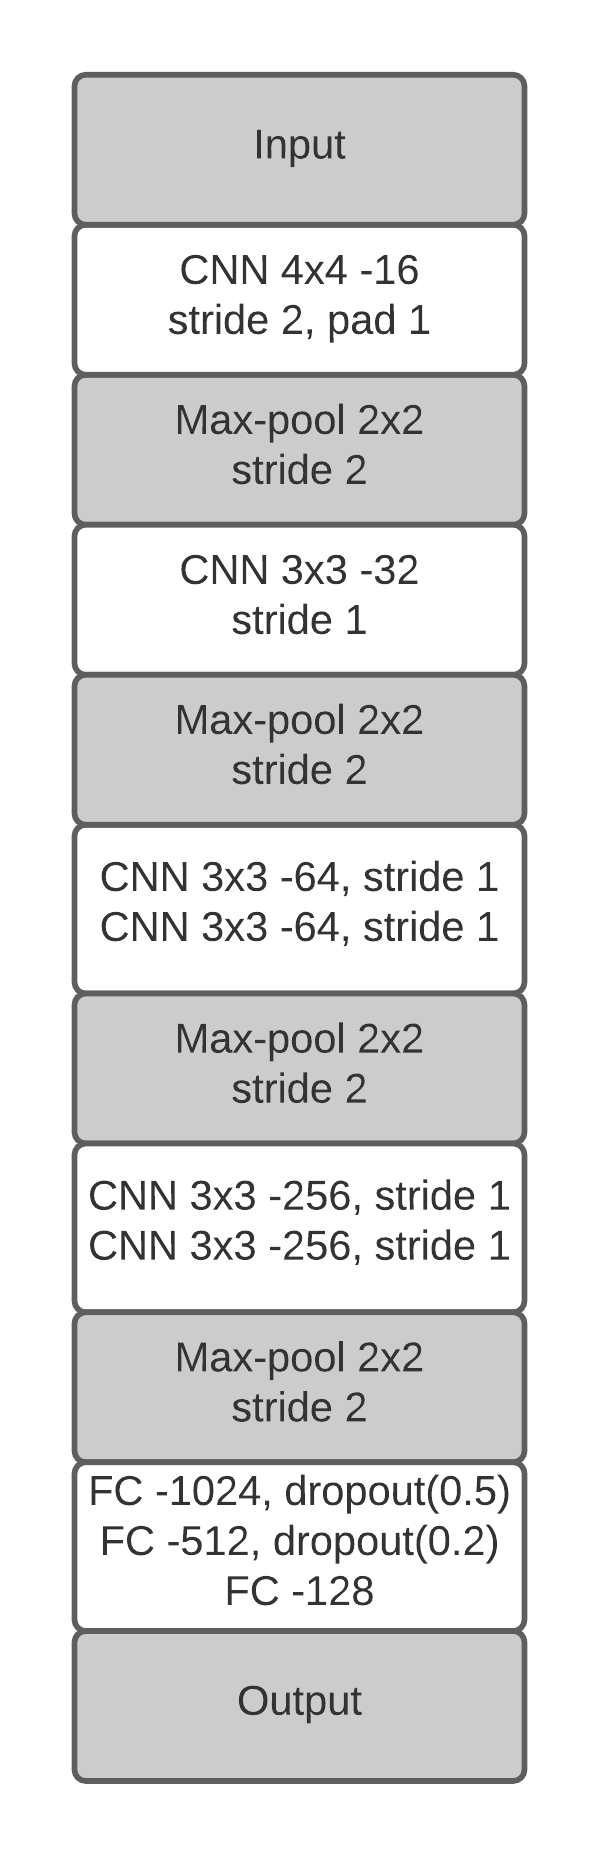
\includegraphics[scale=0.66]{../code/images/Net3_layers.png}
	\caption{Net3}		
	\end{subfigure}
	\begin{subfigure}[t]{.23\textwidth}
		\centering
		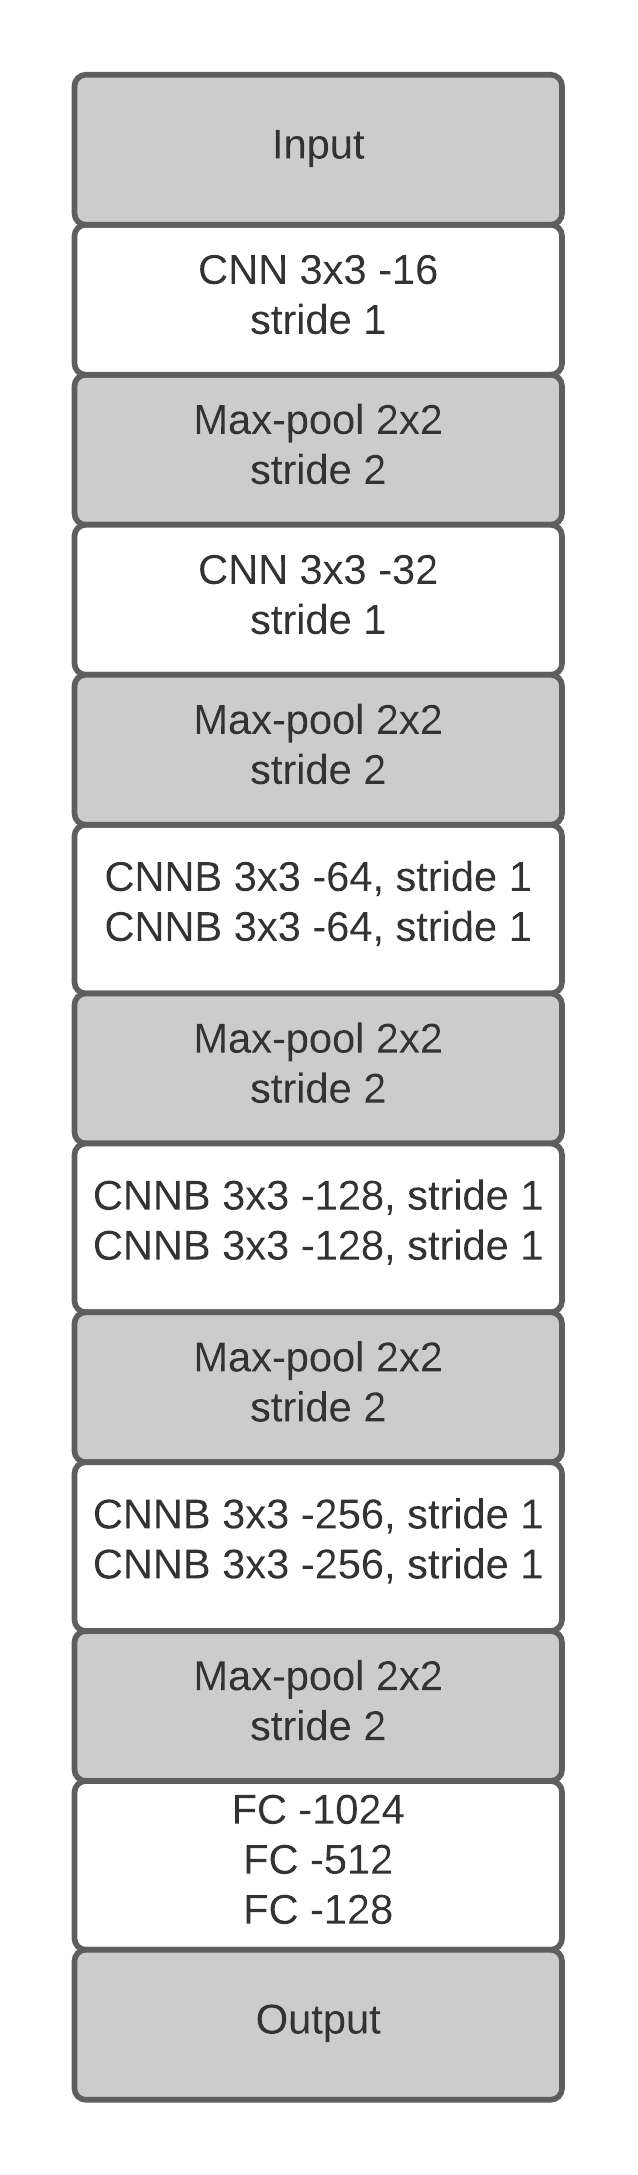
\includegraphics[scale=0.66]{../code/images/Net4_layers.png}
		\caption{Net4}		
		\end{subfigure}
	\caption{Summary of all trained models. CNNB refers to batch normalization before applying ReLU}
	\label{fig:models}
\end{figure}
\clearpage
\subsection{Training Results}
The following accuracy results were obtained after training all $4$ models, which were trained for a total of $50$ epochs. Each model was checkpointed every $10$ epochs, and the model with the best test accuracy was chosen as the final model for Part-B. The accuracies for all models are captured in \cref{table:test-acc}. The loss curve for the best performing model(Net 4) is present in \cref{fig:net4loss}.
\begin{table}[ht]
	\caption{Test and Validation Accuracy Chart(for all 4 models)}% title of Table
	\centering % used for centering table
	\begin{tabular}{|c | c | c | c|}% centered columns (4 columns)
		\hline\hline      
		Model & epochs & validation accuracy(\%) & test accuracy(\%) \\ [0.5ex]
		\hline  
		Net1&              10 &           70.16 &          70.28 \\
			&              20 &           75.88 &          74.64 \\
			&              30 &           78.16 &           76.2 \\
			&              40 &           76.92 &          76.68 \\
			&              50 &            77.8 &          77.16 \\
		\hline
		Net2&              10 &          36.04  &         35.84 \\
			&              20 &          63.12  &         61.44 \\
			&              30 &          73.56  &         70.32 \\
			&              40 &          76.16  &         73.16 \\
			&              50 &           79.4  &         76.16 \\
		\hline
		Net3&              10 &          39.84 &           39.6 \\
			&              20 &           61.2 &           59.4 \\
			&              30 &          70.24 &          69.16 \\
			&              40 &          75.84 &          74.44 \\
			&              50 &          77.32 &          75.48 \\
		\hline
		Net4&              10 &           78.2 &          76.96 \\
			&              20 &           81.4 &          79.92 \\
			&              \textbf{30} &           \textbf{83.4} &          \textbf{82.24} \\
			&              40 &          83.84 &           82.2 \\
			&              50 &          83.48 &          81.96 \\[1ex]
		\hline
	\end{tabular}
	\label{table:test-acc}% is used to refer this table in the text
\end{table}

\begin{figure}[ht]
	\centering
	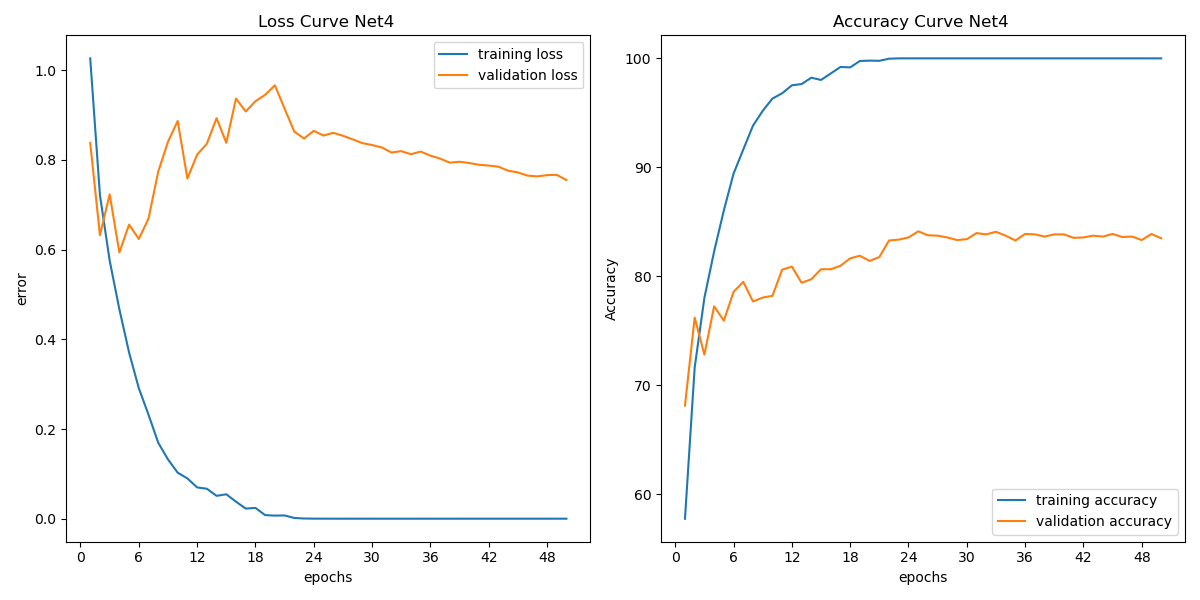
\includegraphics[scale=0.35]{../code/images/Net4.png}
	\caption{Loss curves for Net 4 (best model)}
	\label{fig:net4loss}
\end{figure}

\begin{table}[ht]
	\caption{Classwise accuracy on test dataset for Net4 - $30$ epochs}
	\centering
	\begin{tabular}{|c | c|}
		\hline\hline
		Class & Accuracy(in \%) \\ [0.5ex]
		\hline
		 aeroplane & 96 \\
		       cat & 65 \\
		      deer & 88 \\
		       dog & 70 \\
			  frog & 84 \\ [1ex]
		\hline
	\end{tabular}
\end{table}
\subsection{Training Inferences}
From the figures in \cref{table:test-acc} and the models in \cref{fig:models}, we can make the following conclusions about hyperparameter effects on performance:
\begin{enumerate}
	\item \textbf{Convolutional Layers}: In general, an increase in the number of convolutional layers lead to better train and test accuracy. However, for networks with very large number of conv layers, the train speed is very slow(as evidenced in Net2 and Net3). This can be offset by applying batch normalization after every conv layer(as evidenced in Net4).
	\item \textbf{No of filters/layer}: In general, having more number of filters in higher layers helped capture more detailed features, and led to a higher accuracy(as evidenced in Net3 and Net4)
	\item \textbf{Stride}: Convolving with stride $\geq 1$ seems to result in a reduced accuracy, as evidenced between Net2 and Net3. This happens because we miss out on features when increasing stride.
	\item \textbf{Maxpooling}: Increasing no of maxpooling layers in shallow nets(Net1) leads to greater loss.
\end{enumerate}
In \cref{fig:misclf5}, we can see a small subset of the misclassified images in the dataset split. In most of the images, it is hard to classify the images even with the naked eye.
\begin{figure}[ht]
	\centering
	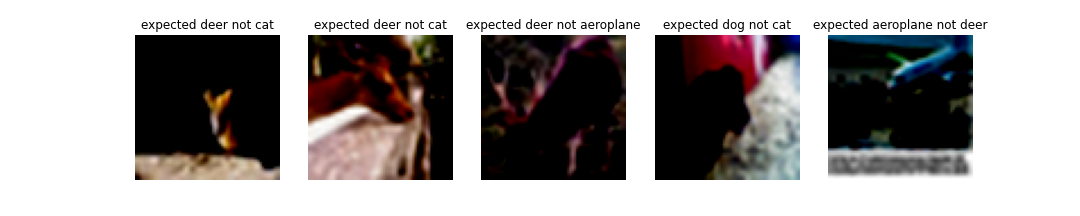
\includegraphics[scale=0.4]{../code/images/misclassified_imgs.png}
	\caption{Some misclassified images}
	\label{fig:misclf5}
\end{figure}

\section{Part-B}
For this part, all experiments are conducted with the weights learned after epoch $30$ of Net4 from Part-A. 
\subsection{Occlusion sensitivity experiment}
Occlusion experiments were carried out on $5$ random samples from the dataset, with a window size of $10 \times 10$ and $20 \times 20$ respectively. Some example images are visualized in \cref{fig:occhmps}.\\
From the heatmap outputs, we can infer that increasing the occlusion kernel size around the main features of the objects to be classified causes the probability of misclassification to increase(increase in blue shading).
\begin{figure}[t]
	\centering
	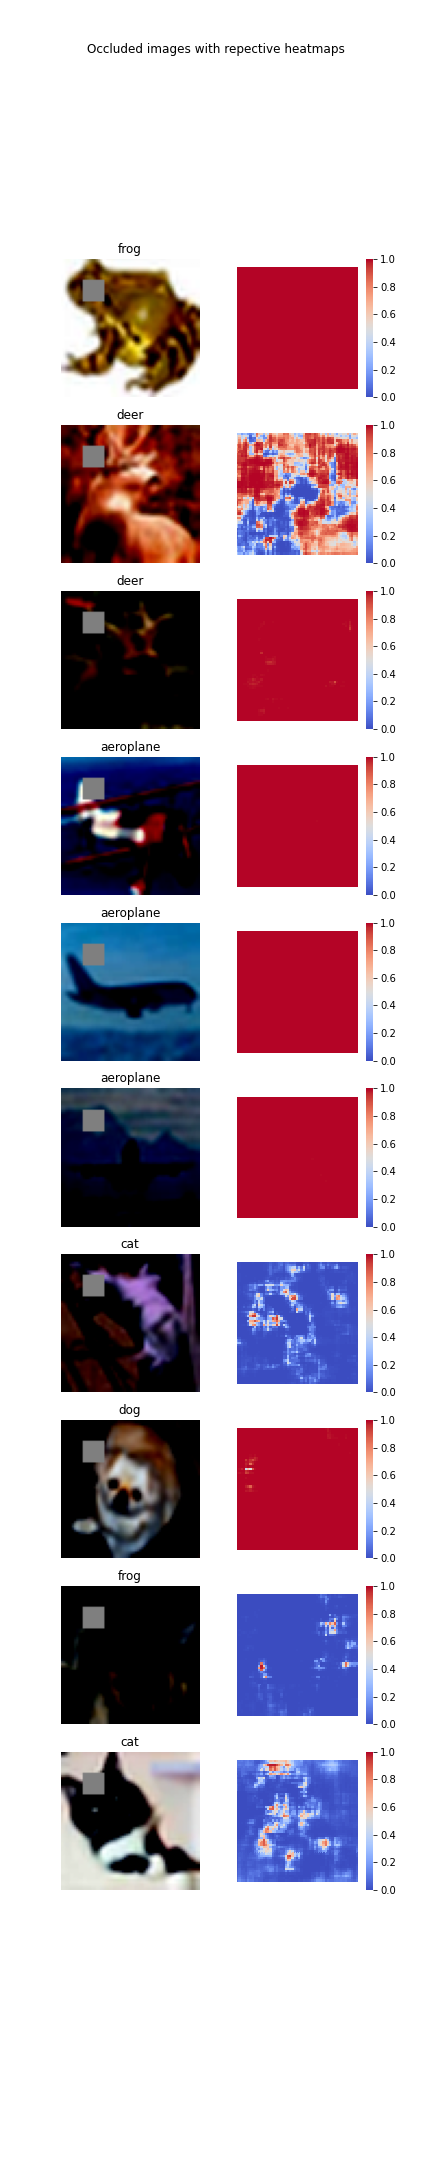
\includegraphics[scale=0.4]{../code/images/Occlusion_heatmaps.png}
	\caption{Images with probability heatmaps for kernels of size $10 \times 10$ and $20 \times 20$ for the occlusion sensitivity experiment}
	\label{fig:occhmps}
\end{figure}
\begin{table}[ht]
	\caption{Filter Selection in Net4}
	\centering
	\begin{tabular}{|c | c|}
		\hline\hline
		Conv Layer(sub-block \#) & Filter \#s \\ [0.5ex]
		\hline
		1 &   2 , 13 \\
		2 &  11 , 23 \\
		3-1 &   9 , 49 \\
		4-1 &  54 , 98 \\
		5-1 &   5 , 171\\ [1ex]
		\hline
	\end{tabular}
	\label{table:filtt}
\end{table}
\pagebreak

\subsection{Filter Analysis}
\subsubsection{Filter Identification}
In Net 4, the filters specified in \cref{table:filtt} were selected for further analysis. Some of these selected filters are visualized in \cref{fig:c1f13} to \cref{fig:c5f171}.

\begin{figure}[h!]
	\centering
	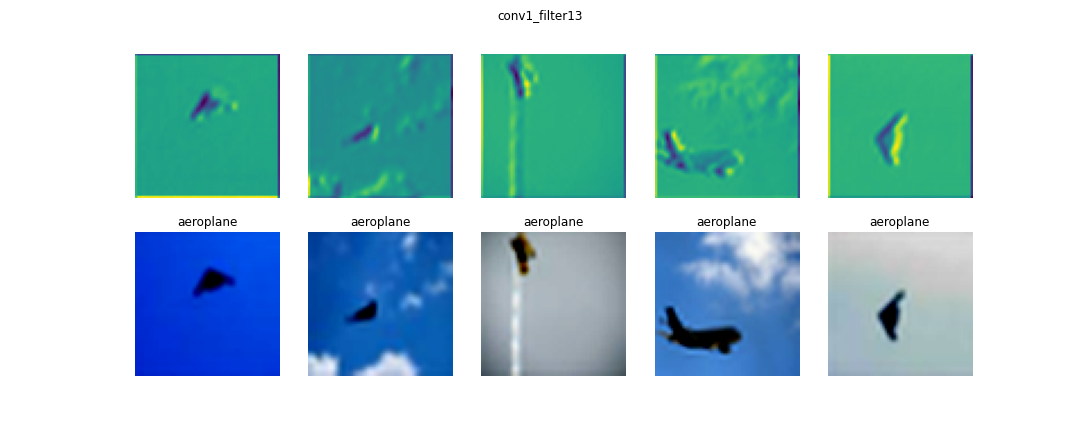
\includegraphics[scale=0.4]{../code/images/Filter_conv1_filter13.png}
	\caption{$13^{th}$ filter output corresponding to $1^{st}$ conv layer of Net4}
	\label{fig:c1f13}
\end{figure}

\begin{figure}[ht]
	\centering
	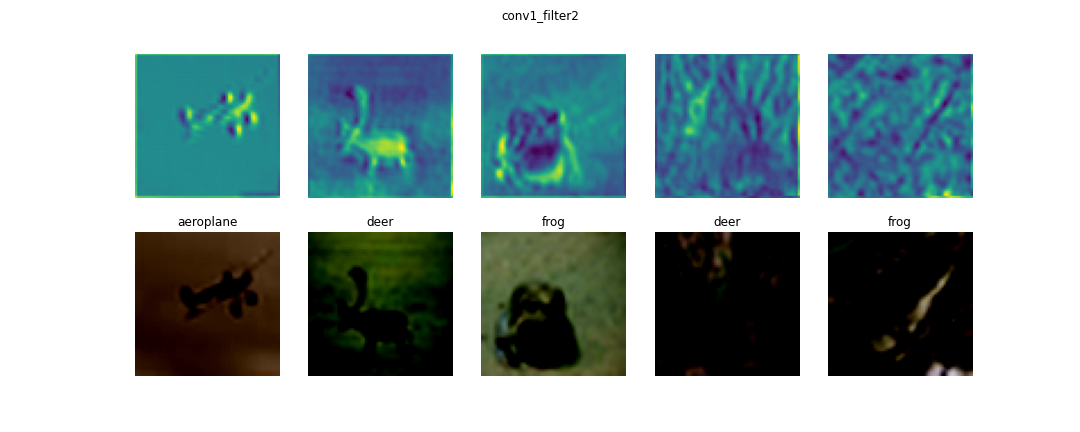
\includegraphics[scale=0.4]{../code/images/Filter_conv1_filter2.png}
	\caption{$2^{nd}$ filter output corresponding to $1^{st}$ conv layer of Net4}
	\label{fig:c1f2}
\end{figure}

\begin{figure}[ht]
	\centering
	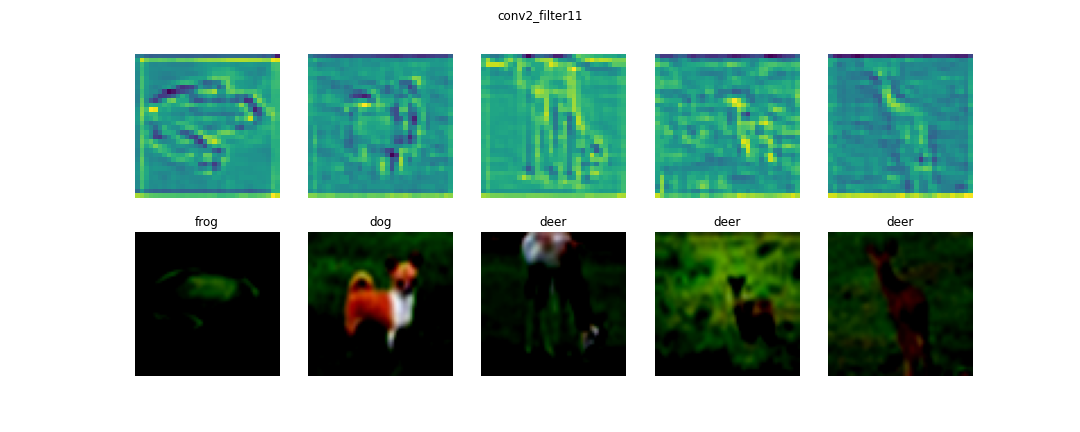
\includegraphics[scale=0.4]{../code/images/Filter_conv2_filter11.png}
	\caption{$12^{th}$ filter output corresponding to $2^{nd}$ conv layer of Net4}
	\label{fig:c2f11}
\end{figure}

\begin{figure}[ht]
	\centering
	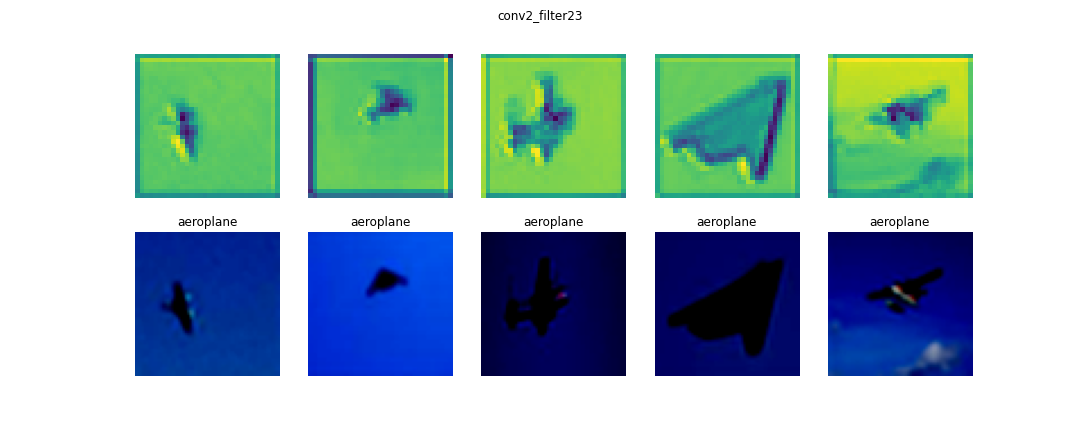
\includegraphics[scale=0.4]{../code/images/Filter_conv2_filter23.png}
	\caption{$23^{rd}$ filter output corresponding to $2^{nd}$ conv layer of Net4}
	\label{fig:c2f23}
\end{figure}

\begin{figure}[ht]
	\centering
	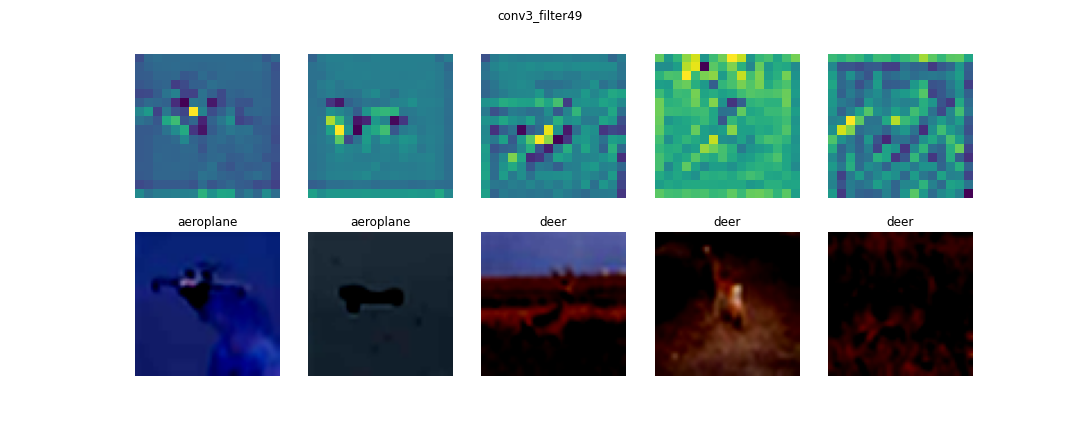
\includegraphics[scale=0.4]{../code/images/Filter_conv3_filter49.png}
	\caption{$49^{th}$ filter output corresponding to $3^{rd}$ conv layer of Net4}
	\label{fig:c3f49}
\end{figure}

\begin{figure}[ht]
	\centering
	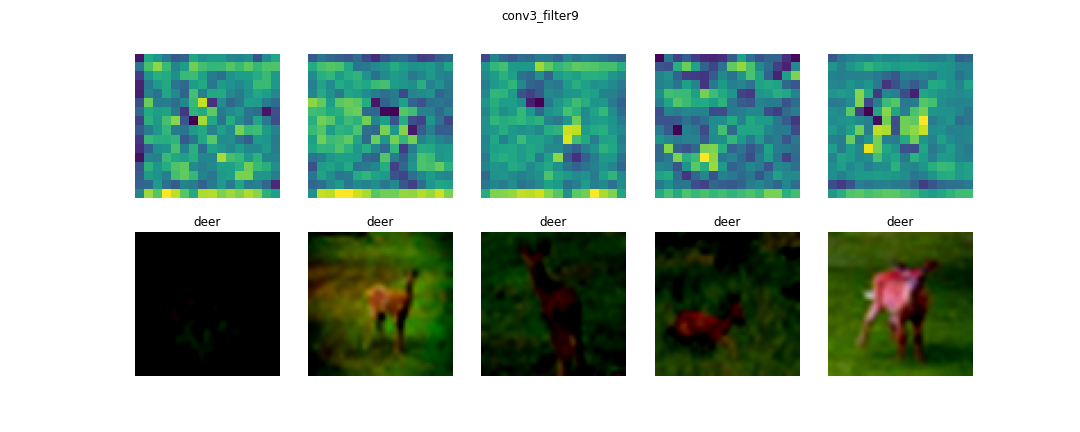
\includegraphics[scale=0.4]{../code/images/Filter_conv3_filter9.png}
	\caption{$9^{th}$ filter output corresponding to $3^{rd}$ conv layer of Net4}
	\label{fig:c3f9}
\end{figure}

\begin{figure}[ht]
	\centering
	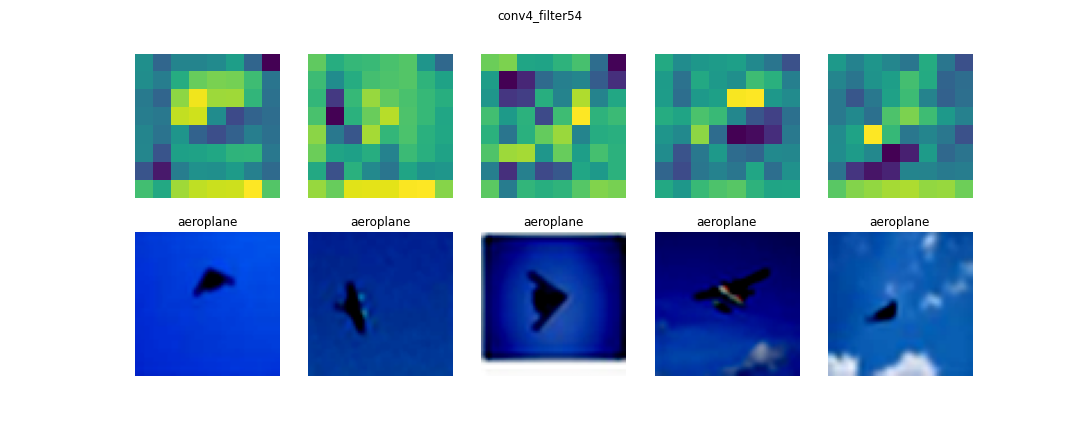
\includegraphics[scale=0.4]{../code/images/Filter_conv4_filter54.png}
	\caption{$4^{th}$ filter output corresponding to $54^{th}$ conv layer of Net4}
	\label{fig:c4f54}
\end{figure}

\begin{figure}[ht]
	\centering
	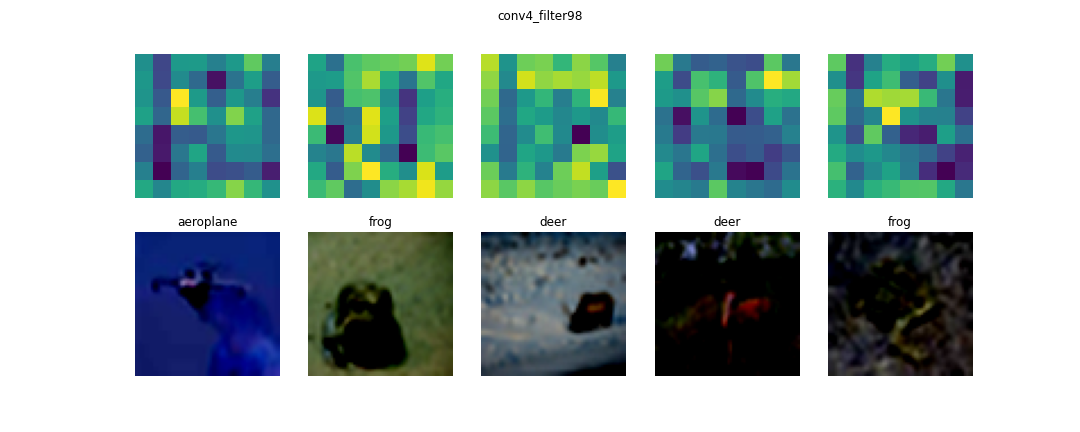
\includegraphics[scale=0.4]{../code/images/Filter_conv4_filter98.png}
	\caption{$4^{th}$ filter output corresponding to $98^{th}$ conv layer of Net4}
	\label{fig:c4f98}
\end{figure}

\begin{figure}[ht]
	\centering
	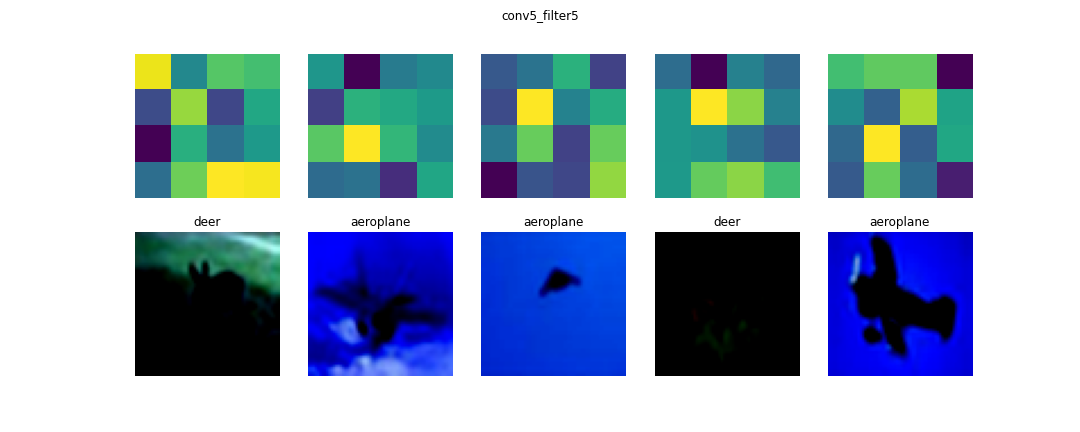
\includegraphics[scale=0.4]{../code/images/Filter_conv5_filter5.png}
	\caption{$5^{th}$ filter output corresponding to $5^{th}$ conv layer of Net4}
	\label{fig:c5f5}
\end{figure}

\begin{figure}[ht]
	\centering
	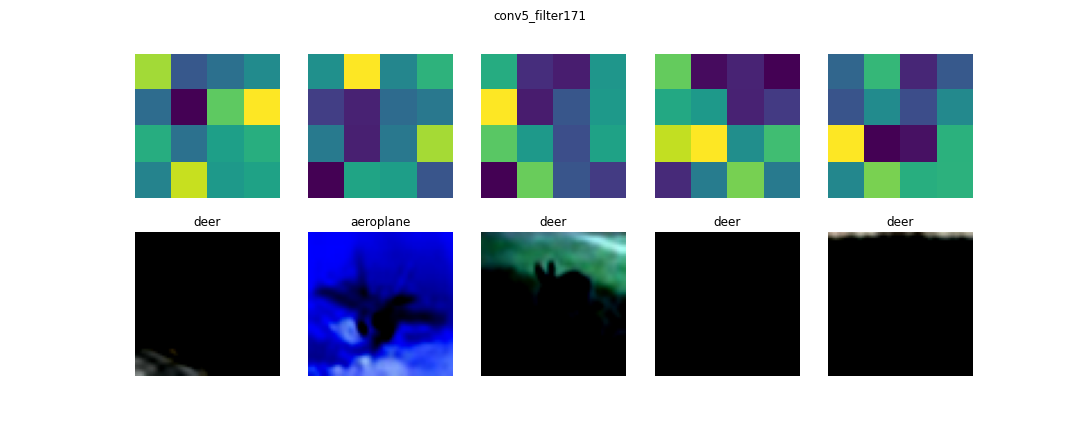
\includegraphics[scale=0.4]{../code/images/Filter_conv5_filter171.png}
	\caption{$171^{st}$ filter output corresponding to $5^{th}$ conv layer of Net4}
	\label{fig:c5f171}
\end{figure}
\clearpage
\subsubsection{Filter Modification}
The stats of the images which mis-classify after switching off the weights of the filters specified in \cref{table:filtt} is captured in \cref{table:miscimgs}\\
\begin{table}[h!]
	\caption{Misclassified image breakup after switching off filters present in \cref{table:filtt}}
	\centering
	\begin{tabular}{|c | c|}
		\hline\hline
		Class & Misclassification count \\ [0.5ex]
		\hline
		 aeroplane & 7 \\
		       cat & 31 \\
		      deer & 18 \\
		       dog & 50 \\
			  frog & 12 \\ [1ex]
		\hline
	\end{tabular}
	\label{table:miscimgs}
\end{table}
By viewing the values in \cref{table:miscimgs}, we can roughly conclude that the net effect of the filters in \cref{table:filtt} is to identify a common feature among cats, dogs and deers, which might be a form of quadrupedalism.\\
\cref{fig:reclfgimgs} shows some of the reclassified images after switching off the weights in \cref{table:filtt}.
\begin{figure}[ht]
	\centering
	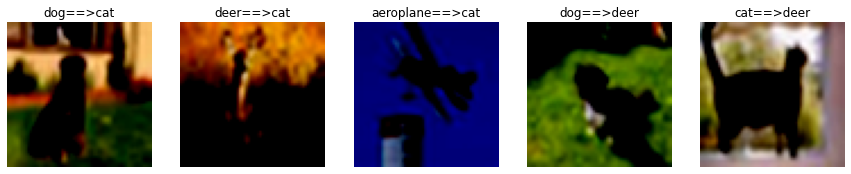
\includegraphics[scale=0.5]{../code/images/misclassified_switchoff.png}
	\caption{Some sample images reclasified after switching off weights}
	\label{fig:reclfgimgs}
\end{figure}
% \section*{Introduction} % Unnumbered section

% Lorem ipsum dolor sit amet, consectetur adipiscing elit. Praesent porttitor arcu luctus, imperdiet urna iaculis, mattis eros. Pellentesque iaculis odio vel nisl ullamcorper, nec faucibus ipsum molestie. Sed dictum nisl non aliquet porttitor. Etiam vulputate arcu dignissim, finibus sem et, viverra nisl. Aenean luctus congue massa, ut laoreet metus ornare in. Nunc fermentum nisi imperdiet lectus tincidunt vestibulum at ac elit. Nulla mattis nisl eu malesuada suscipit.

% % Math equation/formula
% \begin{equation}
% 	I = \int_{a}^{b} f(x) \; \text{d}x.
% \end{equation}

% Aliquam arcu turpis, ultrices sed luctus ac, vehicula id metus. Morbi eu feugiat velit, et tempus augue. Proin ac mattis tortor. Donec tincidunt, ante rhoncus luctus semper, arcu lorem lobortis justo, nec convallis ante quam quis lectus. Aenean tincidunt sodales massa, et hendrerit tellus mattis ac. Sed non pretium nibh. Donec cursus maximus luctus. Vivamus lobortis eros et massa porta porttitor.

% \begin{info} % Information block
% 	This is an interesting piece of information, to which the reader should pay special attention. Fusce varius orci ac magna dapibus porttitor. In tempor leo a neque bibendum sollicitudin. Nulla pretium fermentum nisi, eget sodales magna facilisis eu. Praesent aliquet nulla ut bibendum lacinia. Donec vel mauris vulputate, commodo ligula ut, egestas orci. Suspendisse commodo odio sed hendrerit lobortis. Donec finibus eros erat, vel ornare enim mattis et.
% \end{info}

% %----------------------------------------------------------------------------------------
% %	PROBLEM 1
% %----------------------------------------------------------------------------------------

% \section{Problem title} % Numbered section

% In hac habitasse platea dictumst. Curabitur mattis elit sit amet justo luctus vestibulum. In hac habitasse platea dictumst. Pellentesque lobortis justo enim, a condimentum massa tempor eu. Ut quis nulla a quam pretium eleifend nec eu nisl. Nam cursus porttitor eros, sed luctus ligula convallis quis. Nam convallis, ligula in auctor euismod, ligula mauris fringilla tellus, et egestas mauris odio eget diam. Praesent sodales in ipsum eu dictum.

% %------------------------------------------------

% \subsection{Theoretical viewpoint}

% Maecenas consectetur metus at tellus finibus condimentum. Proin arcu lectus, ultrices non tincidunt et, tincidunt ut quam. Integer luctus posuere est, non maximus ante dignissim quis. Nunc a cursus erat. Curabitur suscipit nibh in tincidunt sagittis. Nam malesuada vestibulum quam id gravida. Proin ut dapibus velit. Vestibulum eget quam quis ipsum semper convallis. Duis consectetur nibh ac diam dignissim, id condimentum enim dictum. Nam aliquet ligula eu magna pellentesque, nec sagittis leo lobortis. Aenean tincidunt dignissim egestas. Morbi efficitur risus ante, id tincidunt odio pulvinar vitae.

% Curabitur tempus hendrerit nulla. Donec faucibus lobortis nibh pharetra sagittis. Sed magna sem, posuere eget sem vitae, finibus consequat libero. Cras aliquet sagittis erat ut semper. Aenean vel enim ipsum. Fusce ut felis at eros sagittis bibendum mollis lobortis libero. Donec laoreet nisl vel risus lacinia elementum non nec lacus. Nullam luctus, nulla volutpat ultricies ultrices, quam massa placerat augue, ut fringilla urna lectus nec nibh. Vestibulum efficitur condimentum orci a semper. Pellentesque ut metus pretium lacus maximus semper. Sed tellus augue, consectetur rhoncus eleifend vel, imperdiet nec turpis. Nulla ligula ante, malesuada quis orci a, ultricies blandit elit.

% % Numbered question, with subquestions in an enumerate environment
% \begin{question}
% 	Quisque ullamcorper placerat ipsum. Cras nibh. Morbi vel justo vitae lacus tincidunt ultrices. Lorem ipsum dolor sit amet, consectetuer adipiscing elit.

% 	% Subquestions numbered with letters
% 	\begin{enumerate}[(a)]
% 		\item Do this.
% 		\item Do that.
% 		\item Do something else.
% 	\end{enumerate}
% \end{question}
	
% %------------------------------------------------

% \subsection{Algorithmic issues}

% In malesuada ullamcorper urna, sed dapibus diam sollicitudin non. Donec elit odio, accumsan ac nisl a, tempor imperdiet eros. Donec porta tortor eu risus consequat, a pharetra tortor tristique. Morbi sit amet laoreet erat. Morbi et luctus diam, quis porta ipsum. Quisque libero dolor, suscipit id facilisis eget, sodales volutpat dolor. Nullam vulputate interdum aliquam. Mauris id convallis erat, ut vehicula neque. Sed auctor nibh et elit fringilla, nec ultricies dui sollicitudin. Vestibulum vestibulum luctus metus venenatis facilisis. Suspendisse iaculis augue at vehicula ornare. Sed vel eros ut velit fermentum porttitor sed sed massa. Fusce venenatis, metus a rutrum sagittis, enim ex maximus velit, id semper nisi velit eu purus.

% \begin{center}
% 	\begin{minipage}{0.5\linewidth} % Adjust the minipage width to accomodate for the length of algorithm lines
% 		\begin{algorithm}[H]
% 			\KwIn{$(a, b)$, two floating-point numbers}  % Algorithm inputs
% 			\KwResult{$(c, d)$, such that $a+b = c + d$} % Algorithm outputs/results
% 			\medskip
% 			\If{$\vert b\vert > \vert a\vert$}{
% 				exchange $a$ and $b$ \;
% 			}
% 			$c \leftarrow a + b$ \;
% 			$z \leftarrow c - a$ \;
% 			$d \leftarrow b - z$ \;
% 			{\bf return} $(c,d)$ \;
% 			\caption{\texttt{FastTwoSum}} % Algorithm name
% 			\label{alg:fastTwoSum}   % optional label to refer to
% 		\end{algorithm}
% 	\end{minipage}
% \end{center}

% Fusce varius orci ac magna dapibus porttitor. In tempor leo a neque bibendum sollicitudin. Nulla pretium fermentum nisi, eget sodales magna facilisis eu. Praesent aliquet nulla ut bibendum lacinia. Donec vel mauris vulputate, commodo ligula ut, egestas orci. Suspendisse commodo odio sed hendrerit lobortis. Donec finibus eros erat, vel ornare enim mattis et.

% % Numbered question, with an optional title
% \begin{question}[\itshape (with optional title)]
% 	In congue risus leo, in gravida enim viverra id. Donec eros mauris, bibendum vel dui at, tempor commodo augue. In vel lobortis lacus. Nam ornare ullamcorper mauris vel molestie. Maecenas vehicula ornare turpis, vitae fringilla orci consectetur vel. Nam pulvinar justo nec neque egestas tristique. Donec ac dolor at libero congue varius sed vitae lectus. Donec et tristique nulla, sit amet scelerisque orci. Maecenas a vestibulum lectus, vitae gravida nulla. Proin eget volutpat orci. Morbi eu aliquet turpis. Vivamus molestie urna quis tempor tristique. Proin hendrerit sem nec tempor sollicitudin.
% \end{question}

% Mauris interdum porttitor fringilla. Proin tincidunt sodales leo at ornare. Donec tempus magna non mauris gravida luctus. Cras vitae arcu vitae mauris eleifend scelerisque. Nam sem sapien, vulputate nec felis eu, blandit convallis risus. Pellentesque sollicitudin venenatis tincidunt. In et ipsum libero. Nullam tempor ligula a massa convallis pellentesque.

% %----------------------------------------------------------------------------------------
% %	PROBLEM 2
% %----------------------------------------------------------------------------------------

% \section{Implementation}

% Proin lobortis efficitur dictum. Pellentesque vitae pharetra eros, quis dignissim magna. Sed tellus leo, semper non vestibulum vel, tincidunt eu mi. Aenean pretium ut velit sed facilisis. Ut placerat urna facilisis dolor suscipit vehicula. Ut ut auctor nunc. Nulla non massa eros. Proin rhoncus arcu odio, eu lobortis metus sollicitudin eu. Duis maximus ex dui, id bibendum diam dignissim id. Aliquam quis lorem lorem. Phasellus sagittis aliquet dolor, vulputate cursus dolor convallis vel. Suspendisse eu tellus feugiat, bibendum lectus quis, fermentum nunc. Nunc euismod condimentum magna nec bibendum. Curabitur elementum nibh eu sem cursus, eu aliquam leo rutrum. Sed bibendum augue sit amet pharetra ullamcorper. Aenean congue sit amet tortor vitae feugiat.

% In congue risus leo, in gravida enim viverra id. Donec eros mauris, bibendum vel dui at, tempor commodo augue. In vel lobortis lacus. Nam ornare ullamcorper mauris vel molestie. Maecenas vehicula ornare turpis, vitae fringilla orci consectetur vel. Nam pulvinar justo nec neque egestas tristique. Donec ac dolor at libero congue varius sed vitae lectus. Donec et tristique nulla, sit amet scelerisque orci. Maecenas a vestibulum lectus, vitae gravida nulla. Proin eget volutpat orci. Morbi eu aliquet turpis. Vivamus molestie urna quis tempor tristique. Proin hendrerit sem nec tempor sollicitudin.

% % File contents
% \begin{file}[hello.py]
% \begin{lstlisting}[language=Python]
% #! /usr/bin/python

% import sys
% sys.stdout.write("Hello World!\n")
% \end{lstlisting}
% \end{file}

% Fusce eleifend porttitor arcu, id accumsan elit pharetra eget. Mauris luctus velit sit amet est sodales rhoncus. Donec cursus suscipit justo, sed tristique ipsum fermentum nec. Ut tortor ex, ullamcorper varius congue in, efficitur a tellus. Vivamus ut rutrum nisi. Phasellus sit amet enim efficitur, aliquam nulla id, lacinia mauris. Quisque viverra libero ac magna maximus efficitur. Interdum et malesuada fames ac ante ipsum primis in faucibus. Vestibulum mollis eros in tellus fermentum, vitae tristique justo finibus. Sed quis vehicula nibh. Etiam nulla justo, pellentesque id sapien at, semper aliquam arcu. Integer at commodo arcu. Quisque dapibus ut lacus eget vulputate.

% % Command-line "screenshot"
% \begin{commandline}
% 	\begin{verbatim}
% 		$ chmod +x hello.py
% 		$ ./hello.py

% 		Hello World!
% 	\end{verbatim}
% \end{commandline}

% Vestibulum sodales orci a nisi interdum tristique. In dictum vehicula dui, eget bibendum purus elementum eu. Pellentesque lobortis mattis mauris, non feugiat dolor vulputate a. Cras porttitor dapibus lacus at pulvinar. Praesent eu nunc et libero porttitor malesuada tempus quis massa. Aenean cursus ipsum a velit ultricies sagittis. Sed non leo ullamcorper, suscipit massa ut, pulvinar erat. Aliquam erat volutpat. Nulla non lacus vitae mi placerat tincidunt et ac diam. Aliquam tincidunt augue sem, ut vestibulum est volutpat eget. Suspendisse potenti. Integer condimentum, risus nec maximus elementum, lacus purus porta arcu, at ultrices diam nisl eget urna. Curabitur sollicitudin diam quis sollicitudin varius. Ut porta erat ornare laoreet euismod. In tincidunt purus dui, nec egestas dui convallis non. In vestibulum ipsum in dictum scelerisque.

% % Warning text, with a custom title
% \begin{warn}[Notice:]
%   In congue risus leo, in gravida enim viverra id. Donec eros mauris, bibendum vel dui at, tempor commodo augue. In vel lobortis lacus. Nam ornare ullamcorper mauris vel molestie. Maecenas vehicula ornare turpis, vitae fringilla orci consectetur vel. Nam pulvinar justo nec neque egestas tristique. Donec ac dolor at libero congue varius sed vitae lectus. Donec et tristique nulla, sit amet scelerisque orci. Maecenas a vestibulum lectus, vitae gravida nulla. Proin eget volutpat orci. Morbi eu aliquet turpis. Vivamus molestie urna quis tempor tristique. Proin hendrerit sem nec tempor sollicitudin.
% \end{warn}

% %----------------------------------------------------------------------------------------


\end{document}
